
\documentclass[
11pt, % The default document font size, options: 10pt, 11pt, 12pt
%codirector, % Uncomment to add a codirector to the title page
]{charter}




% El títulos de la memoria, se usa en la carátula y se puede usar el cualquier lugar del documento con el comando \ttitle
\titulo{Solución IoT para robot de exploración ambiental de datos críticos con almacenamiento en blockchain}

% Nombre del posgrado, se usa en la carátula y se puede usar el cualquier lugar del documento con el comando \degreename
\posgrado{Carrera de Maestría en Internet de las Cosas}
%\posgrado{Carrera de Especialización en Internet de las Cosas}
%\posgrado{Carrera de Especialización en Intelegencia Artificial}
%\posgrado{Maestría en Sistemas Embebidos}
%\posgrado{Maestría en Internet de las cosas}

% Tu nombre, se puede usar el cualquier lugar del documento con el comando \authorname
\autor{Ing. Gonzalo F. Carreño}

% El nombre del director y co-director, se puede usar el cualquier lugar del documento con el comando \supname y \cosupname y \pertesupname y \pertecosupname
\director{Esp. Ing. Sergio Alberino}
\pertenenciaDirector{UTN.BA}
% FIXME:NO IMPLEMENTADO EL CODIRECTOR ni su pertenencia
%\codirector{CODIRECTOR} % para que aparezca en la portada se debe descomentar la opción codirector en el documentclass
%\pertenenciaCoDirector{FIUBA}

% Nombre del cliente, quien va a aprobar los resultados del proyecto, se puede usar con el comando \clientename y \empclientename
\cliente{Esp. Lic. Mariano Landini}
\empresaCliente{FCE UBA - Cliente}

% Nombre y pertenencia de los jurados, se pueden usar el cualquier lugar del documento con el comando \jurunoname, \jurdosname y \jurtresname y \perteunoname, \pertedosname y \pertetresname.
\juradoUno{Nombre y Apellido (1)}
\pertenenciaJurUno{pertenencia (1)}
\juradoDos{Nombre y Apellido (2)}
\pertenenciaJurDos{pertenencia (2)}
\juradoTres{Nombre y Apellido (3)}
\pertenenciaJurTres{pertenencia (3)}
\fechaINICIO{1 de julio de 2024}		%Fecha de inicio de la cursada de GdP \fechaInicioName
\fechaFINALPlan{1 de junio de 2025} 	%Fecha de final de cursada de GdP
\fechaFINALTrabajo{20 de octubre de 2025}	%Fecha de defensa pública del trabajo final


\begin{document}

\maketitle
\thispagestyle{empty}
\pagebreak


\thispagestyle{empty}
{\setlength{\parskip}{0pt}
\tableofcontents{}
}
\pagebreak


\section*{Registros de cambios}
\label{sec:registro}


\begin{table}[ht]
\label{tab:registro}
\centering
\begin{tabularx}{\linewidth}{@{}|c|X|c|@{}}
\hline
\rowcolor[HTML]{C0C0C0}
Revisión & \multicolumn{1}{c|}{\cellcolor[HTML]{C0C0C0}Detalles de los cambios realizados} & Fecha      \\ \hline
0      & Creación del documento.                                 &\fechaInicioName \\ \hline


\end{tabularx}
\end{table}

\pagebreak



\section*{Acta de constitución del proyecto}
\label{sec:acta}

\begin{flushright}
Buenos Aires, \fechaInicioName
\end{flushright}

\vspace{2cm}

Por medio de la presente se acuerda con el \authorname\hspace{1px} que su Trabajo Final de la \degreename\hspace{1px} se titulará ``\ttitle'', consistirá en \textcolor{black}{la implementación de un sistema embebido de robot de exploración ambiental conectado a un sistema back-end en la nube pública capaz de persistir los datos en una red blockhain}, y tendrá un presupuesto preliminar estimado de \textcolor{black}{\$ 160} dólares estadounidenses y \textcolor{black}{721} horas de trabajo, con fecha de inicio \fechaInicioName\hspace{1px} y fecha de presentación pública estimada \fechaFinalName.

Se adjunta a esta acta la planificación inicial.

\vfill

% Esta parte se construye sola con la información que hayan cargado en el preámbulo del documento y no debe modificarla
\begin{table}[ht]
\centering
\begin{tabular}{ccc}
\begin{tabular}[c]{@{}c@{}}Dr. Ing. Ariel Lutenberg \\ Director posgrado FIUBA\end{tabular} & \hspace{2cm} & \begin{tabular}[c]{@{}c@{}}\clientename \\ \empclientename \end{tabular} \vspace{2.5cm} \\
\multicolumn{3}{c}{\begin{tabular}[c]{@{}c@{}} \supname \\ Director del Trabajo Final\end{tabular}} \vspace{2.5cm} \\
%\begin{tabular}[c]{@{}c@{}}\jurunoname \\ Jurado del Trabajo Final\end{tabular}     &  & \begin{tabular}[c]{@{}c@{}}\jurdosname\\ Jurado del Trabajo Final\end{tabular}  \vspace{2.5cm}  \\
%\multicolumn{3}{c}{\begin{tabular}[c]{@{}c@{}} \jurtresname\\ Jurado del Trabajo Final\end{tabular}} \vspace{.5cm}                                                                    
\end{tabular}
\end{table}




\section{1. Descripción técnica-conceptual del proyecto a realizar}
\label{sec:descripcion}

\begin{consigna}{black} % El bloque "consigna" se usa para poner texto en rojo y dar una pequeña ayuda sobre cómo completar la sección. En cada entrega parcial deben eliminar los comandos begin y end del bloque consigna de las secciones que hayan completado.
El presente proyecto es un emprendimiento personal que busca integrar el dispositivo robótico de exploración ambiental controlable a distancia desarrollado en el marco de la carrera de especialización en sistemas embebidos con un backend para el análisis y explotación de datos en la nube pública y una red blockchain para el almacenamiento inmutable de datos críticos.

\textit{\textbf{Estado del arte:}}
Los robots exploradores son los dispositivos robotizados que han sido creados con el fin de reconocer y explorar un lugar o terreno siendo capaces de moverse de forma autónoma o controlados por personas a control remoto. Su objetivo es evitar poner en riesgo la vida de los humanos, ya sea debido a que el lugar es inaccesible o porque se encuentra en una zona contaminada.
Algunos de los tipos de robots exploradores más conocidos son los espaciales, de minas, de rescate en catástrofes, de tuberías, acuáticos y/o submarinos, y de suelos.

Estos dispositivos, forman parte de una solución arquitectónica IoT más amplia, cumpliendo el rol de nodos “edge”.  Una vez implementados y funcionando envían lecturas del reconocimiento y operaciones realizadas a sistemas de procesamiento y almacenamiento de datos que conforman el backend, generalmente en la nube, desde donde se puede visualizar los resultados obtenidos, sus métricas derivadas, realizar trazabilidad de las operaciones así como almacenar y gobernar los datos generados.

En situaciones en las que el robot es utilizado para explorar y monitorear un área ambientalmente sensible, como una reserva natural o un sitio afectado por un desastre ecológico y su misión es recopilar datos críticos -como niveles de contaminación, temperatura, humedad, y calidad del aire- es de gran importancia almacenar estas mediciones de una forma en la que se pueda asegurar la integridad y transparencia de los datos, como por ejemplo, en una cadena de bloques (blockchain).

Una arquitectura blockchain se basa en el procesamiento y almacenamiento de transacciones agrupadas en bloques encadenados e inmutables de forma distribuida entre los nodos de una red en lo que se conoce como un distributed ledger. De esta manera se puede asegurar integridad de los datos ya que los registros generados no se pueden modificar una vez creados. Además, como la red es accesible entre los actores intervinientes en el caso de uso -pudiendo ser pública o privada y con o sin permisos-, se puede garantizar la transparencia de los datos.
La mayoría de las redes blockchain constan de la tecnología para la implementación de código backend ejecutable en la red, que aunque su nombre puede cambiar dependiendo de la red en la cual se implementan, usualmente se los conoce como Smart Contracts. La ejecución de estos componentes es realizada por los nodos de la red en el proceso que se conoce como minería, y como tal es una actividad que requiere el pago de un fee conocido como gas medido en diferentes unidades dependiendo de la red y normalmente pagable desde una cuenta nominada en el token de la red asociada a la aplicación o propietario de los smart contracts.
La  forma de interactuar con los smart contracts en un caso de uso interactivo desde afuera de la red, se realiza a través de otro componente conocido como dApps (de-centralized applications) que haciendo uso de ciertas librerías de Web3 invocan a estos para almacenar y obtener datos en y desde el ledger.

En el siguiente diagrama se puede apreciar una posible arquitectura del sistema final.



\begin{center}
  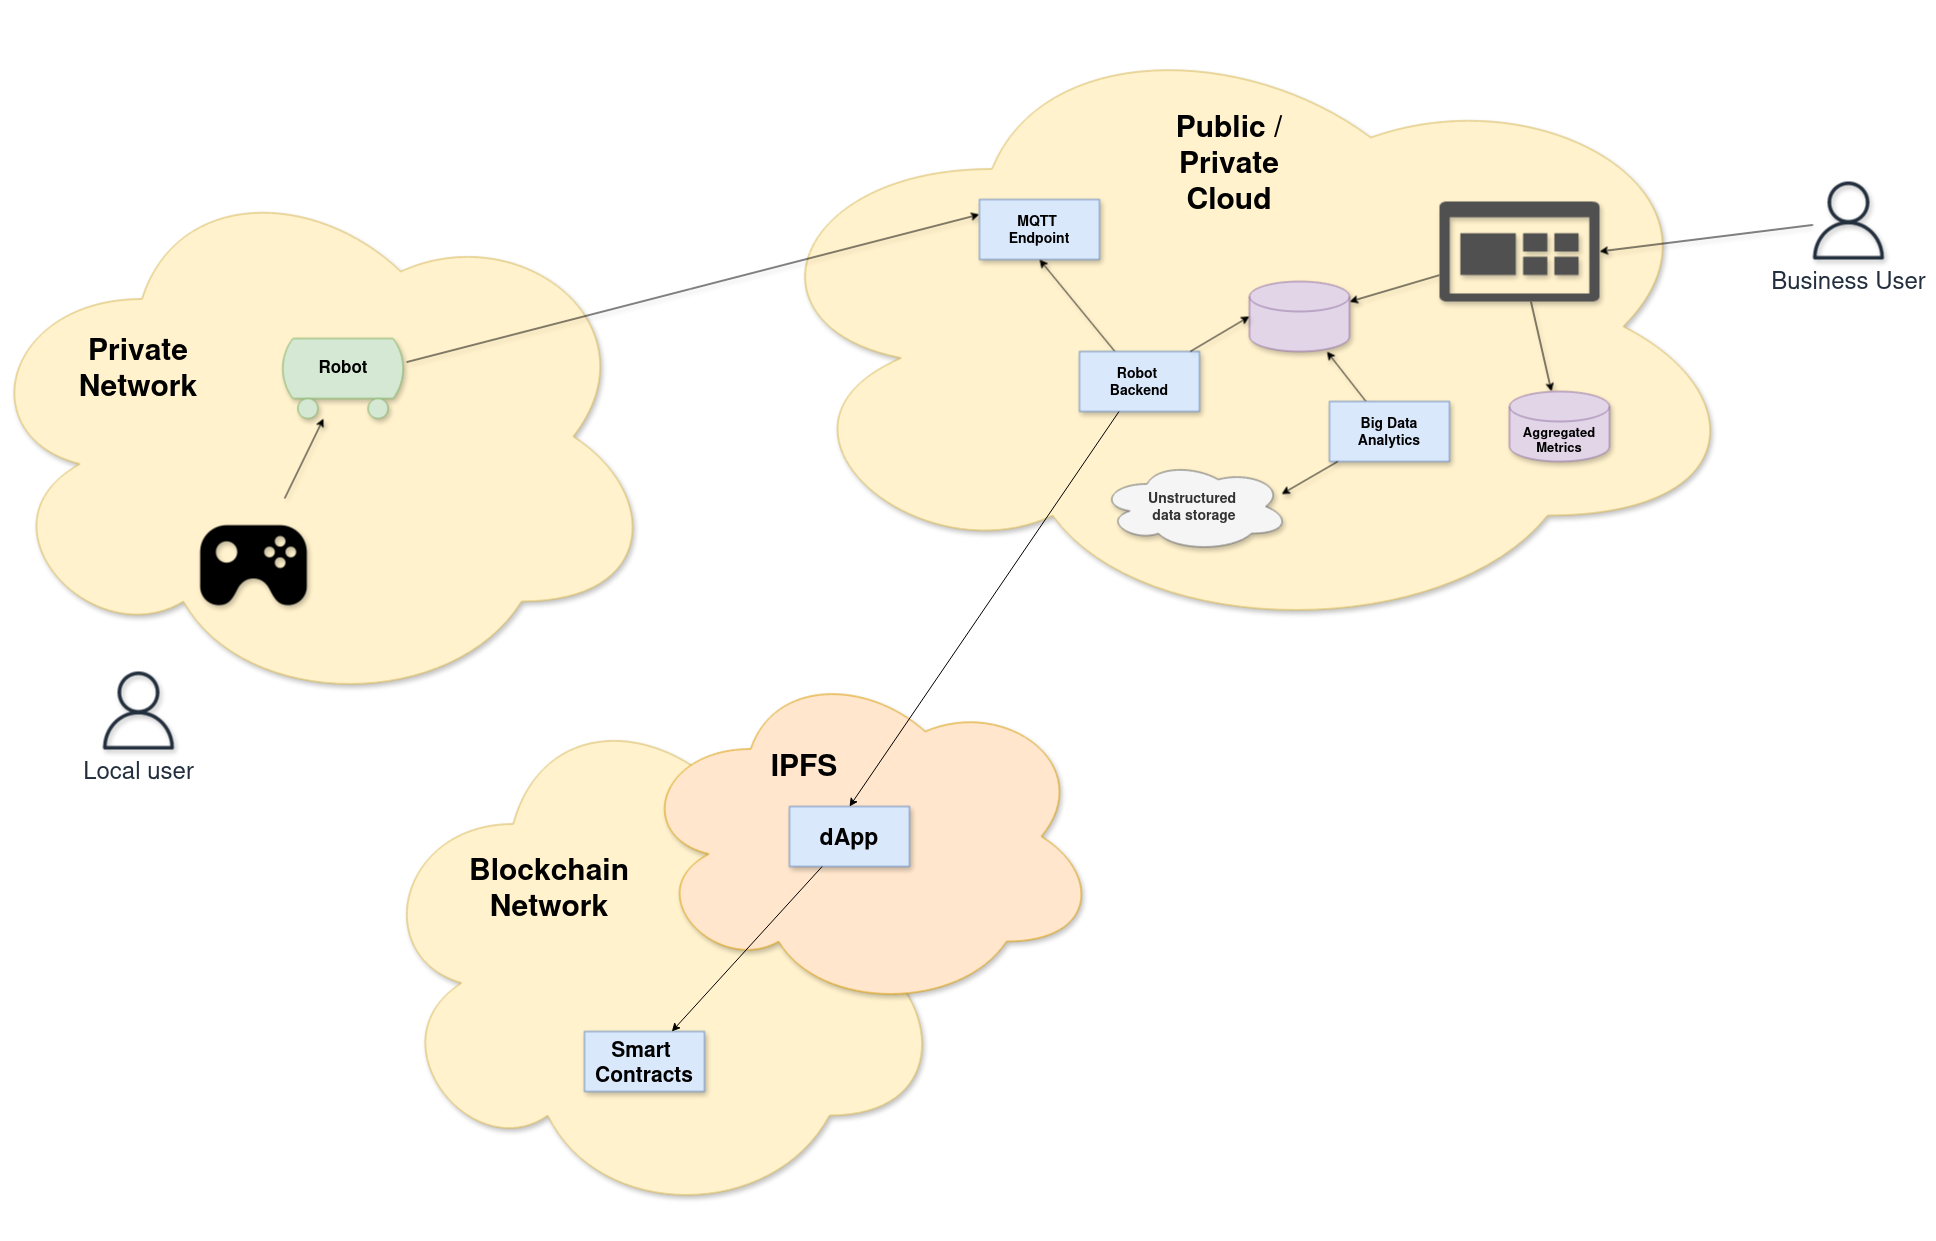
\includegraphics[scale=0.15]{Figuras/IoTProject-Page-1.drawio}
  \captionof{figure}{Arquitectura del sistema}
  \label{fig:esp32}
\end{center}




El hardware utilizado para la solución de IoT propuesta es un robot de exploración ambiental de control inalámbrico, desarrollado en la Carrera de Especialización en Sistemas Embebidos de la Universidad de Buenos Aires. En la siguiente imagen puede apreciarse una fotografía del mismo.

\begin{center}
  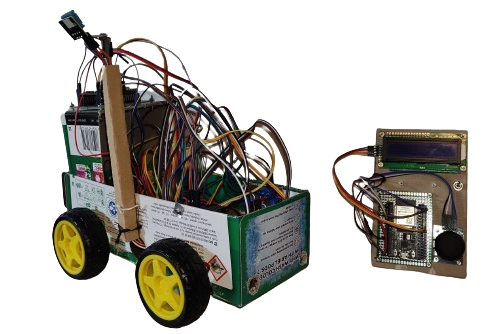
\includegraphics[scale=0.5]{Figuras/Robot_y_Joystick_1}
  \captionof{figure}{Arquitectura del sistema}
  \label{fig:esp32}
\end{center}




\vspace{25px}


\end{consigna}

\section{2. Identificación y análisis de los interesados}
\label{sec:interesados}
\begin{consigna}{black} % este comando se debe borrar para la entrega, junto con la contraparte \end{consigna}{red}
A continuación se enumeran los diferentes roles e individuos que participarán en el proyecto.
\begin{table}[ht]
%\caption{Identificación de los interesados}
%\label{tab:interesados}
\begin{tabularx}{\linewidth}{@{}|l|l|X|l|@{}}
\hline
\rowcolor[HTML]{C0C0C0}
Rol           & Nombre y Apellido & Organización 	& Puesto 	\\ \hline

Cliente       & \clientename      &\empclientename	&  -      	\\ \hline
Responsable   & \authorname       & UTN.BA        	& Alumno 	\\ \hline
Orientador    & \supname	      & \pertesupname 	& Director Trabajo final \\ \hline
\end{tabularx}
\end{table}


\end{consigna} % este comando se debe borrar para la entrega, junto con la contraparte \begin{consigna}{red}



\section{3. Propósito del proyecto}
\label{sec:proposito}

\begin{consigna}{black}
El propósito de este proyecto es desarrollar una solución IoT para un robot de exploración ambiental para casos de uso de datos críticos en los que sea necesario contar con almacenamiento inmutable y transparente para todas las partes en una arquitectura blockchain
Por otra parte, se pretende volcar en un desarrollo concreto y de aplicación industrial los conocimientos adquiridos durante la cursada de la Maestria en Internet de las Cosas.

\end{consigna}

\section{4. Alcance del proyecto}
\label{sec:alcance}

\begin{consigna}{black}
Contando con el hardware mencionado anteriormente que auspicia de componente edge en una arquitectura IoT, se propone la implementación de la plataforma tecnológica que alcanza:

\begin{itemize}
	\item La publicación del endpoint MQTT para la recepción de los datos enviados por el robot.
	\item La adaptación del sistema embebido del robot de exploración ambiental para la conexión segura con el backend vía MQTT.
	\item La arquitectura e implementación de los sistemas backend y el modelo de datos necesario para el almacenamiento de las mediciones enviadas por el robot.
	\item La arquitectura, implementación y despliegue de la dApp (de-centralized application) y Smart Contracts necesarios para el almacenamiento de las mediciones en una red Blockchain (a definir).
	\item La definición de métricas agregadas de valor y posterior arquitectura e implementación de los sistemas analíticos para procesar de forma batch y/o real-time (dependiendo de las métricas a definir) los datos enviados utilizando herramientas de procesamiento paralelo basadas en big data.
	\item La implementación de la interfaz gráfica para poder visualizar los datos enviados y analíticas calculadas.

\end{itemize}


\end{consigna}


\section{5. Supuestos del proyecto}
\label{sec:supuestos}

\begin{consigna}{black}
Para el desarrollo del presente proyecto se supone que:

\begin{itemize}
	\item será posible tener acceso a redes de desarrollo y testing de forma gratuita mediante la obtención de Faucets,
	\item será posible experimentar, desarrollar y hacer testing del backend cloud con el presupuesto estimado,
	\item arquitectónicamente resultará viable implementar la solución propuesta,
	\item se dispondrá del conjunto de librerías, drivers y APIs de bajo nivel para el desarrollo de las funcionalidades planteadas en el alcance sin ser necesario el desarrollo de drivers y dichos componentes de bajo nivel. Además, tanto estos componentes de software como los open source de la comunidad de software libre utilizados durante el desarrollo del producto, se encontrará estable para que su integración en el proyecto no resulte en desvíos,	
	\item tanto el prototipado de los componentes de software del sistema embebido como el ensamblado de los componentes de hardware del dispositivo no producirán desvíos considerables en el plan,
	\item no habrá desvíos no contemplados en el plan que impidan o demoren entregas en el proyecto,
	\item el comité académico encargado de la corrección tendrá disponibilidad para realizar la evaluación en las fechas planificadas de entrega,
	\item el director asignado tendrá la disponibilidad de tiempo para darle seguimiento al proyecto,
	\item el alumno contará con una disponibilidad de entre 3 y 5 horas diarias (incluyendo fines de semana) para el desarrollo del proyecto en el tiempo convenido,
	\item los materiales, componentes, software de terceros y servicios cloud utilizados funcionaran de forma óptima y de acuerdo a lo esperado,
	\item el robot desarrollado seguirá funcionando de forma estable sin ser necesario su ajuste, reparacion o modificacion a nivel hardware o sistema base (fuera de lo planificado para la integración con MQTT),
	\item los recursos no directamente relacionados con el desarrollo del proyecto, pero utilizados durante el mismo, funcionaran adecuadamente y en caso de falta de suministro (por ejemplo el servicio de internet) o avería (por ejemplo en el caso de la computadora utilizada) la resolución será expeditiva no suponiendo un desvío en el plan,
	\item no sucederán nuevos eventos de impacto global (pandemia, guerras, etc) durante el desarrollo del proyecto que impliquen una demora o imposibilidad en la entrega.
\end{itemize}


\end{consigna}

\section{6. Requerimientos}
\label{sec:requerimientos}
\begin{consigna}{black}
A continuación se listan los requerimientos del producto:

\begin{enumerate}	
	\item Requerimientos funcionales		
	\begin{enumerate}	
		
		\item El robot de exploración ambiental debe poder enviar a la plataforma datos de mediciones de parámetros ambientales, incluyendo los datos de fecha, hora, localización geográfica (puede ser implementada como un mock inicialmente) y la categorización si es o no un valor crítico.
		\item El robot de exploración ambiental debe incorporar lógica para categorizar los valores medidos de cada parámetro ambiental como valores críticos si:
		\begin{enumerate}				
			\item representan un maximo o minimo global sensado hasta el momento,				
			\item representan un máximo o mínimo local durante el último día.				
		\end{enumerate}			
		\item La plataforma debe poder recibir y almacenar las mediciones de parámetros ambientales enviadas por el robot.
		\item La plataforma debe poder procesar las mediciones de parámetros ambientales enviadas por el robot para generar métricas de valor para el usuario de negocio.		
		\item El la plataforma proveer dos front-end con interfaz web:
			\begin{enumerate}				
				\item el front-end para el usuario de negocio,				
				\item el front-end para el usuario administrador.				
			\end{enumerate}			
		
		\item El front-end para el usuario de negocio debe proveer métricas para visualizar:
			\begin{enumerate}				
				\item las lecturas históricas almacenadas,				
				\item agregaciones (máximo, mínimo, promedio, etc) de cada parámetro ambiental agrupado por frecuencias (ventanas de tiempo) y coordenadas geográficas,				
				\item las referencias a los datos persistidos en blockchain.
			\end{enumerate}			
		\item El front-end para el usuario de administración debe permitir:
			\begin{enumerate}				
				\item acceder a los diferentes recursos utilizados por la herramienta (topics MQTT, smart contracts, buckets, etc),
				\item resetear valores y estado.			
			\end{enumerate}			
		\end{enumerate}	

					
	\item Requerimientos no funcionales		
	\begin{enumerate}	
		\item La plataforma debe contar con al menos un backend de procesamiento y acceso a datos operacionales para la lógica de negocio.
		\item La plataforma debe contar con al menos un backend de acceso, procesamiento, almacenamiento de datos analytics para la  generación de métricas.		
		\item El envío de los valores ambientales censados al backend debe ser mediante MQTT.
		\item Las lecturas ambientales categorizadas como críticas deben ser almacenadas en blockchain para garantizar fiable, inmutabilidad.
		\item La gestión de datos almacenados en blockchain debe ser implementada mediante smart contracts desplegados en la red.
		\item La interacción con los smart contracts debe realizarse desde una dApp.
		\item Los sistemas de transferencia y almacenamiento de datos utilizados deben contar con seguridad, permitiendo encriptación, autenticación y autorización.	
		\end{enumerate}	
		
	\item Requerimientos de documentación		
		\begin{enumerate}			
			\item documentación de arquitectura técnica a alto nivel del diseño del sistema.			
			\item documentación técnica de la implementación del software.
			\item manual de usuario.	
			\item memoria final.	
		\end{enumerate}	
	\item Requerimiento de testing		
		\begin{enumerate}			
			\item se debe incluir tests de unitarios de componentes,
			\item se debe incluir tests funcionales (smoke test) del producto general.		
		\end{enumerate}	
	
	\item Requerimientos opcionales		
		\begin{enumerate}			
			\item De infraestructura y despliegue:
				\begin{enumerate}			
					\item se permite realizar el despliegue de la dApp en un IPFS (preferentemente) o en la nube.					
					\item se permite agregado hardware al robot para la captura de datos adicionales.
					\item se permite agregar automatización para la creación de la infraestructura como código.
				\end{enumerate}			
			
			\item De datos:
				\begin{enumerate}			
					\item se permite almacenar cualquier otro dato adicional sensado o derivado.
					\item se permite agregar cualquier implementación de gobierno de datos.	
					\item se permite almacenar cualquier otra métrica o gráfico de explotación de datos adicional.
				\end{enumerate}
		
	\end{enumerate}
\end{enumerate}
\end{consigna}

\section{7. Historias de usuarios (\textit{Product backlog})}
\label{sec:backlog}

\begin{consigna}{black}
A continuación se listan las historias de usuario. La ponderación de \textit{story points} se realiza considerando 1 punto = 1 hora:


\begin{enumerate}

	\item Métricas agregadas
	\begin{itemize}
		\item Detalle: Como usuario quiero una métrica que me indique los valores agregados de mínimo, máximo y promedio de cada parámetro ambiental agrupado por fecha y coordenadas.
		\item Esfuerzo: 24 puntos
		\item Criterio de aceptación: funcionalidad verificada (incluyendo prototipado, integración y ensamblado), tests y documentación.
	\end{itemize}
	
	\item Métricas históricas
	\begin{itemize}
		\item Detalle: Como usuario quiero poder ver en series de tiempo los valores medidos para los diferentes parámetros ambientales.
		\item Esfuerzo: 24 puntos
		\item Criterio de aceptación: funcionalidad verificada (incluyendo prototipado, integración y ensamblado), tests y documentación.
	\end{itemize}
	
	\item Gráficos de explotación
	\begin{itemize}
		\item Detalle: Como usuario quiero contar con métricas gráficas (heatmap, pie, etc) para poder visualizar más fácilmente los agregados.
		\item Esfuerzo: 24 puntos
		\item Criterio de aceptación: funcionalidad verificada (incluyendo prototipado, integración y ensamblado), tests y documentación.
	\end{itemize}
	
	\item Smart contracts
	\begin{itemize}
		\item Detalle: Como arquitecto quiero que el acceso a los datos en blockchain se realice por medio de la implementación de smart contracts.
		\item Esfuerzo: 24 puntos
		\item Criterio de aceptación: funcionalidad verificada (incluyendo prototipado, integración y ensamblado), tests y documentación.
	\end{itemize}
	
	\item dApp
	\begin{itemize}
		\item Detalle: Como arquitecto quiero que el acceso a los smart contracts se realice desde una dApp utilizando una biblioteca Web3.
		\item Esfuerzo: 24 puntos
		\item Criterio de aceptación: funcionalidad verificada (incluyendo prototipado, integración y ensamblado), tests y documentación.
	\end{itemize}
	
	\item Integración MQTT
	\begin{itemize}
		\item Detalle: Como arquitecto quiero que el envío de los datos desde el robot al backend se realice mediante MQTT.
		\item Esfuerzo: 24 puntos
		\item Criterio de aceptación: funcionalidad verificada (incluyendo prototipado, integración y ensamblado), tests y documentación.
	\end{itemize}


	\item Arquitectura operacional
	\begin{itemize}
		\item Detalle: Como arquitecto quiero que la arquitectura de tanto los front-ends como el back-end sean web exponiendo APIs vía servicios REST. La interfaz gráfica debe ser implementada en Angular u otro framework MVC/MVVC de Javascript.
		\item Esfuerzo: 24 puntos
		\item Criterio de aceptación: funcionalidad verificada (incluyendo prototipado, integración y ensamblado), tests y documentación.
	\end{itemize}

	\item Arquitectura analitica
	\begin{itemize}
		\item Detalle: Como arquitecto quiero que las métricas de valor sean generadas de forma batch mediante un pipeline de datos.
		\item Esfuerzo: 24 puntos
		\item Criterio de aceptación: funcionalidad verificada (incluyendo prototipado, integración y ensamblado), tests y documentación.
	\end{itemize}

	\item Encriptación punto a punto
	\begin{itemize}
		\item Detalle: Como ingeniero de seguridad quiero que los datos transmitidos en cada segmento viajen encriptados mediante certificados.
		\item Esfuerzo: 24 puntos
		\item Criterio de aceptación: funcionalidad verificada (incluyendo prototipado, integración y ensamblado), tests y documentación.
	\end{itemize}
	
\end{enumerate}
\end{consigna}



\section{8. Entregables principales del proyecto}
\label{sec:entregables}
\begin{consigna}{black}
Los entregables del proyecto son:
\begin{itemize}
	\item Video demostrativo del uso de la plataforma. 		
	\item Código fuente del firmware.
	\item Código fuente del software.
	\item Documentación:
	\begin{enumerate}				
		\item Manual de usuario,			
		\item Memoria final,
		\item Documentación de arquitectura técnica del sistema (hardware y software),
	\end{enumerate}	
	

\end{itemize}
\end{consigna}

\section{9. Desglose del trabajo en tareas}
\label{sec:wbs}

\begin{consigna}{black}
El conjunto de actividades y tareas que se realizarán durante el proyecto son:


\end{consigna}

\section{10. Diagrama de Activity On Node}
\label{sec:AoN}

\begin{consigna}{black}
A continuación se detalla la lista de actividades que se realizarán durante el proyecto. Los tiempos están expresados en días, y como se considera una dedicación de 4 horas diarias (incluyendo fines de semana).

\begin{table}[ht]
%\caption{Identificación de los interesados}
%\label{tab:interesados}
\begin{tabularx}{\linewidth}{@{}|l|X|l|l|l|@{}}
\hline
\rowcolor[HTML]{C0C0C0}
Id	& Tarea           						& Duración 	& Dependencia	& Predecesora 	\\ \hline
1	& Set-up integración continua (opcional)	& 11d  		& -        		&  -				\\ \hline
2	& Desarrollo cloud						& 70d		& -				&  -      		\\ \hline
3	& Desarrollo blockchain    				& 60d			& -			 	& -			\\ \hline
4	& Gestión del proyecto 					& 40d		& -				&  - 			\\ \hline
5	& Documentación    						& 42d		& -			 	& -				\\ \hline

\end{tabularx}
\end{table}

Como se puede apreciar en la figura \ref{fig:activityOnNode}, el camino crítico está formado por la tarea [2] \textit{(desarrollo cloud)} y su duración es 70 días.

\begin{center}
  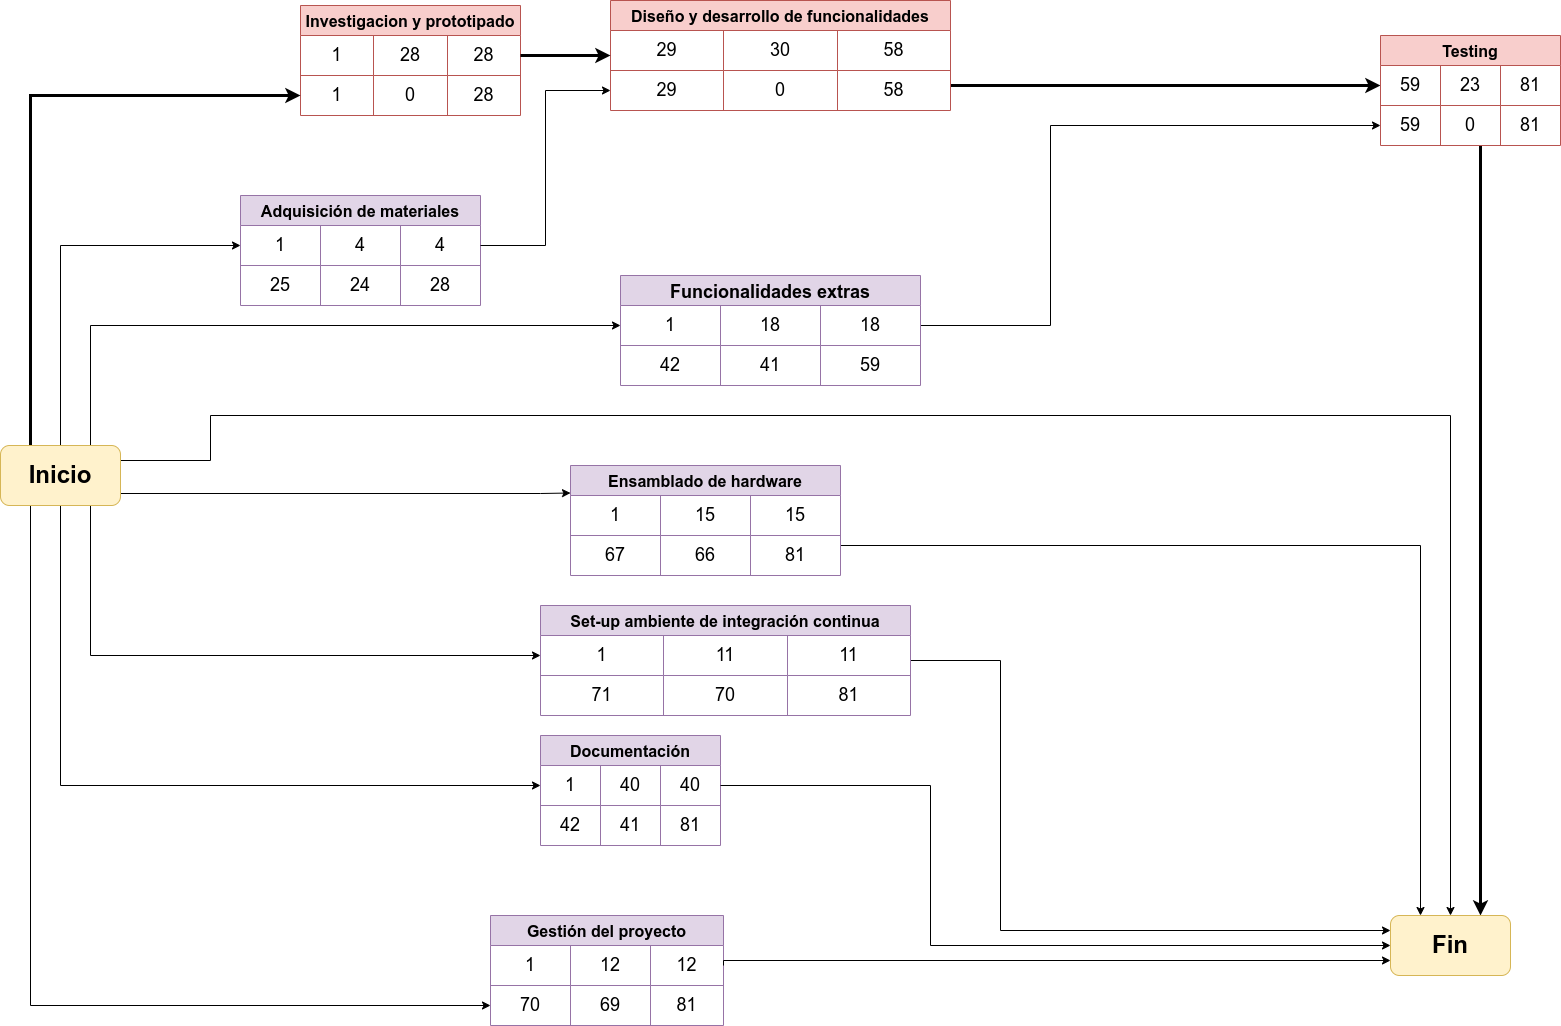
\includegraphics[scale=0.30]{./Figuras/activity-on-node}
  \captionof{figure}{Diagrama de \textit{Activity-On-Node}.}
  \label{fig:activityOnNode}
\end{center}

\end{consigna}


\section{11. Diagrama de Gantt}
\label{sec:gantt}

\begin{consigna}{black}


\begin{figure}[htpb]
\centering
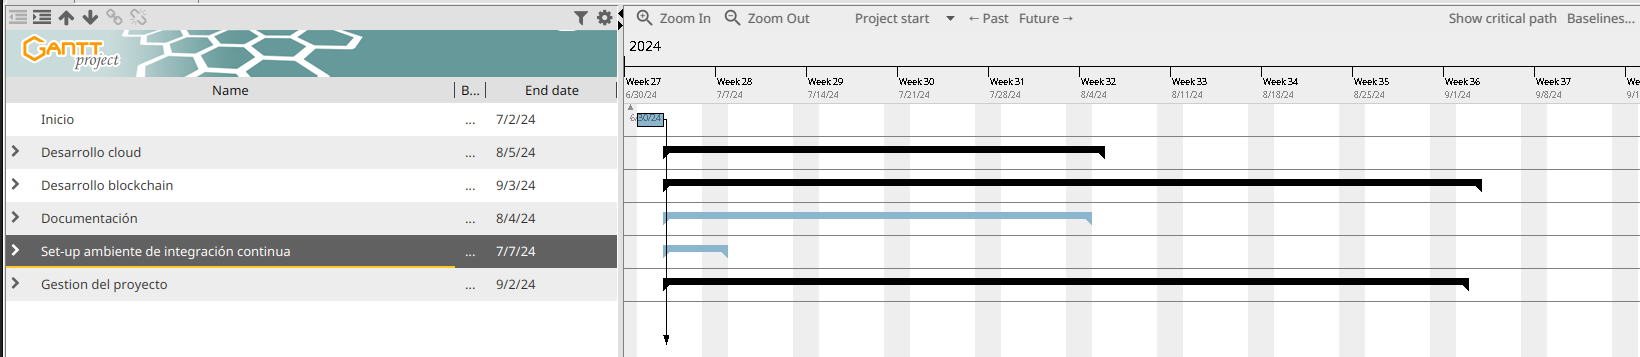
\includegraphics[width=.9\textwidth]{./Figuras/gantt-0}
\caption{Diagrama de \textit{Gantt} general.}
\label{fig:diagBloques}
\end{figure}

\begin{figure}[htpb]
\centering
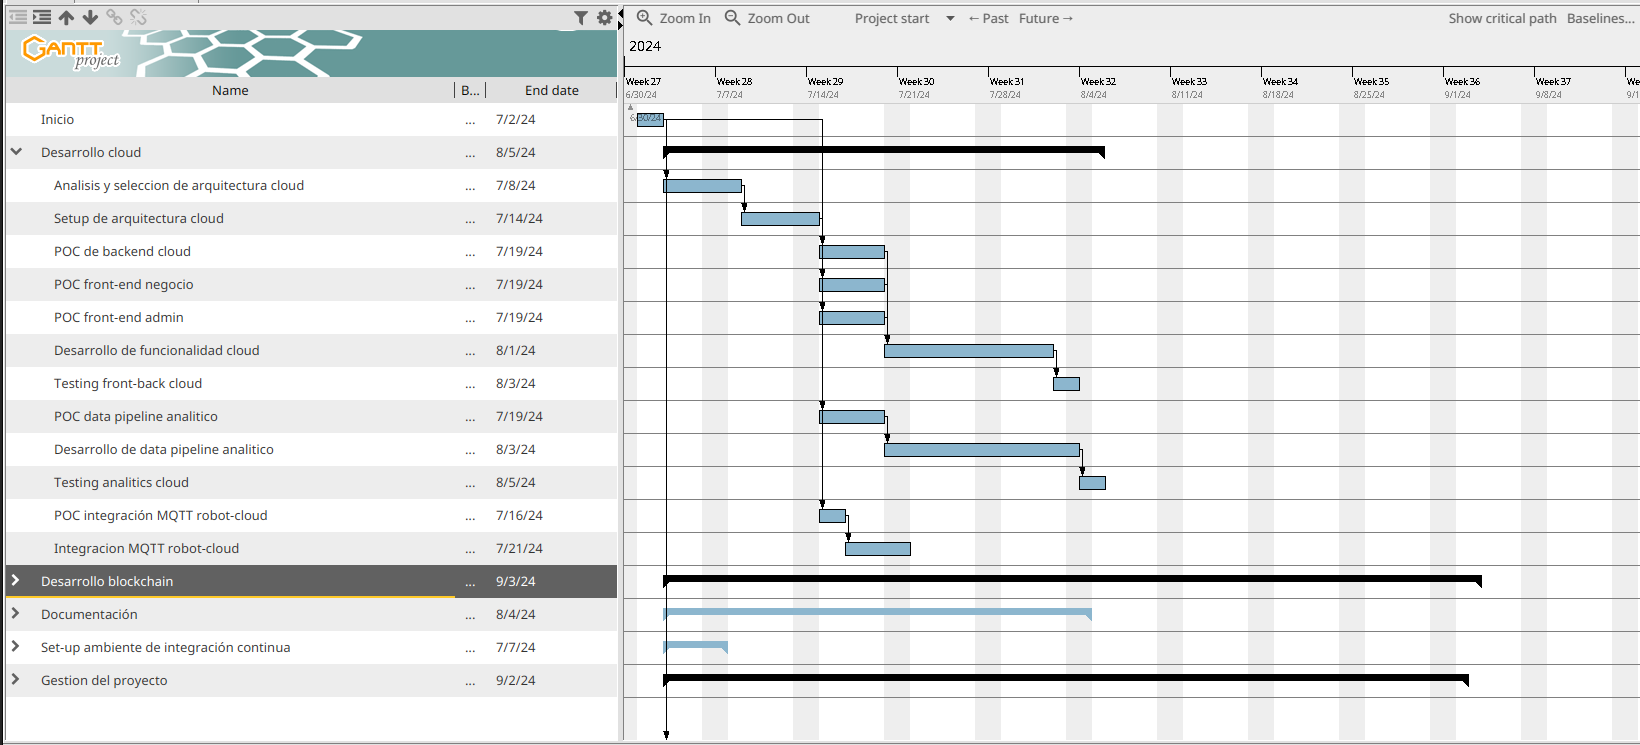
\includegraphics[width=.9\textwidth]{./Figuras/gantt-1}
\caption{Diagrama de \textit{Gantt} detallado (parte 1).}
\label{fig:diagBloques}
\end{figure}


\begin{figure}[htpb]
\centering
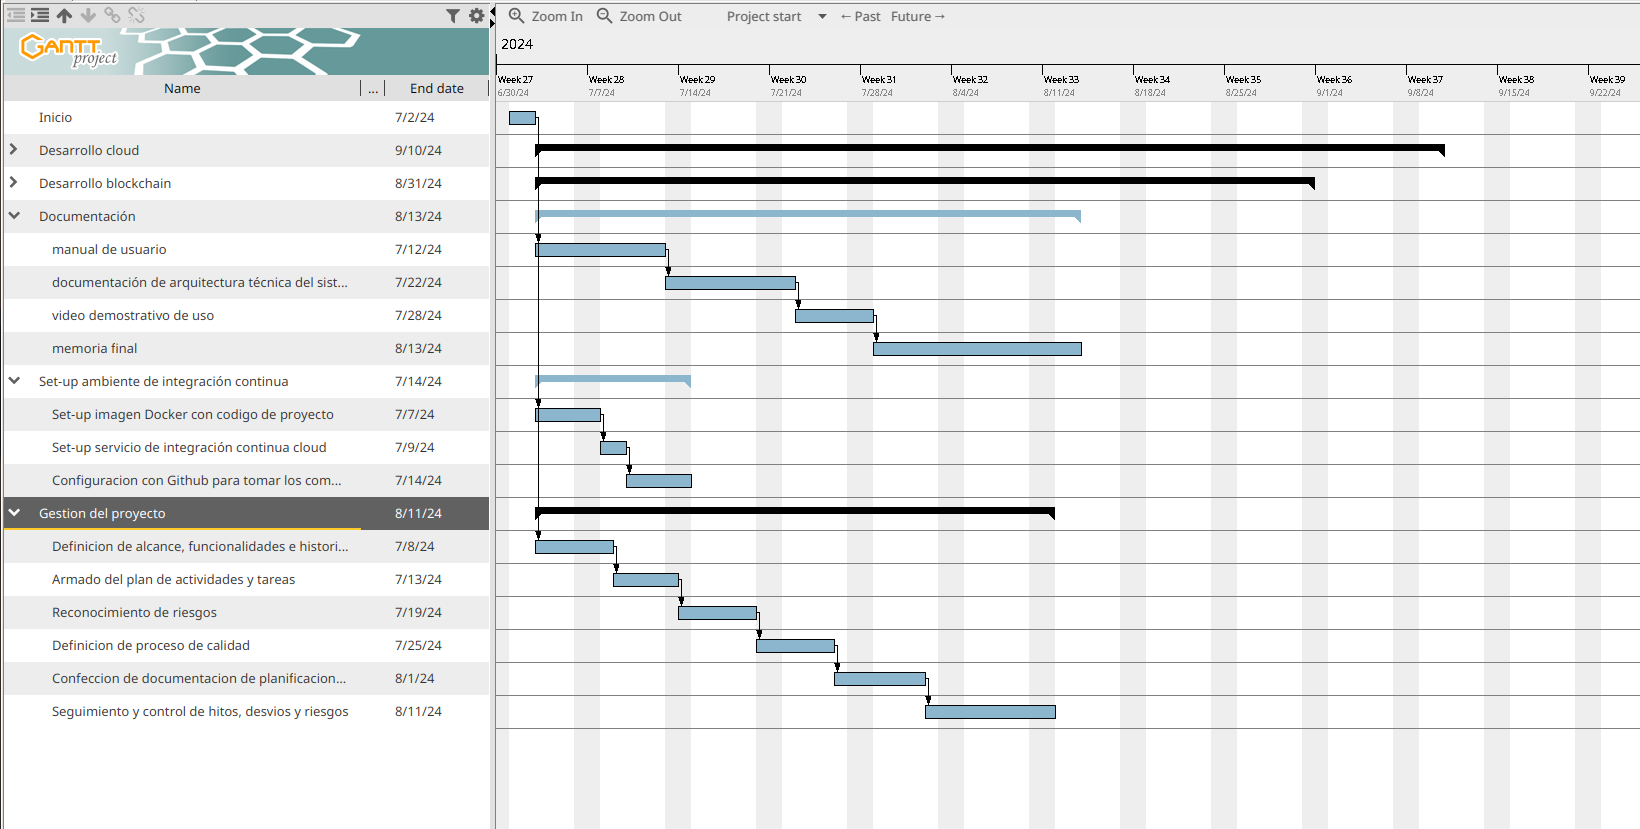
\includegraphics[width=.9\textwidth]{./Figuras/gantt-2}
\caption{Diagrama de \textit{Gantt} detallado (parte 2).}
\label{fig:diagBloques}
\end{figure}
\end{consigna}

\section{12. Presupuesto detallado del proyecto}
\label{sec:presupuesto}

\begin{consigna}{black}
El siguiente cuadro presenta los costos en dólares estadounidenses estimados para el proyecto:

\end{consigna}

\begin{table}[htpb]
\centering
\begin{tabularx}{\linewidth}{@{}|X|c|r|r|@{}}
\hline
\rowcolor[HTML]{C0C0C0}
\multicolumn{4}{|c|}{\cellcolor[HTML]{C0C0C0}COSTOS DIRECTOS} \\ \hline
\rowcolor[HTML]{C0C0C0}
Descripción &
 \multicolumn{1}{c|}{\cellcolor[HTML]{C0C0C0}Cantidad} &
 \multicolumn{1}{c|}{\cellcolor[HTML]{C0C0C0}Valor unitario} &
 \multicolumn{1}{c|}{\cellcolor[HTML]{C0C0C0}Valor total} \\ \hline
Procesamiento cloud &
 \multicolumn{1}{c|}{1} &
 \multicolumn{1}{c|}{\$ 50,00} &
 \multicolumn{1}{c|}{\$ 50,00} \\ \hline
Almacenamiento cloud &
 \multicolumn{1}{c|}{1} &
 \multicolumn{1}{c|}{\$ 20,00} &
 \multicolumn{1}{c|}{\$ 20,00} \\ \hline
Transferencia de datos cloud &
 \multicolumn{1}{c|}{1} &
 \multicolumn{1}{c|}{\$ 50,00} &
 \multicolumn{1}{c|}{\$ 50,00} \\ \hline
Alojamiento IPFS &
 \multicolumn{1}{c|}{1} &
 \multicolumn{1}{c|}{\$ 20,00} &
 \multicolumn{1}{c|}{\$ 20,00} \\ \hline
Varios &
 \multicolumn{1}{c|}{1} &
 \multicolumn{1}{c|}{\$ 20,00} &
 \multicolumn{1}{c|}{\$ 20,00} \\ \hline
\rowcolor[HTML]{C0C0C0}
\multicolumn{3}{|c|}{TOTAL} &
 \multicolumn{1}{c|}{\$ 160,00} \\ \hline
\end{tabularx}%
\end{table}


\section{13. Gestión de riesgos}
\label{sec:riesgos}
\begin{consigna}{black}

\begin{enumerate}

\item Riesgo de demora
\begin{itemize}
	\item Severidad (S): 9 - Teniendo en cuenta que solo habrá un recurso (el alumno) asignado al proyecto desarrollando el producto, una demora en cualquier tarea puede implicar demora en la fecha de entrega.
	\item Ocurrencia (O): 5 - Dado el desafío de innovación planteado por el alcance él la probabilidad de demora es media.
\end{itemize}


\item Riesgo de no contar con toda la funcionalidad deseada
\begin{itemize}
	\item Severidad (S): 9 - El no cumplimiento con la funcionalidad deseada pone en riesgo el éxito del proyecto.
	\item Ocurrencia (O): 5 - Dado el desafío de innovación planteado por el alcance el la probabilidad de no contar con toda la funcionalidad es media.
\end{itemize}

\item Riesgo de calidad insuficiente
\begin{itemize}
	\item Severidad (S): 4 - La calidad insuficiente no pone en riesgo el cumplimiento con la funcionalidad pero si compromete la estabilidad y resistencia a fallas del producto, por lo que puede desencadenar en un producto poco o menos confiable.
	\item Ocurrencia (O): 4 - Se estima que con las técnicas empleadas durante el desarrollo del producto, este riesgo tiene una baja probabilidad de ocurrencia.
\end{itemize}


\item Riesgo de desvío en costos
\begin{itemize}
	\item Severidad (S): 5 - La ocurrencia de este riesgo impacta en los costos del proyecto, pero no imposibilita ni demora la entrega del producto.
	\item Ocurrencia (O): 8 - Teniendo en cuenta que los precios son estimados sin haber cerrado la definición de la arquitectura final y la inflación argentina, es muy probable que exista un desvío en costos.
\end{itemize}

\item Riesgo de indisponibilidad de recursos
\begin{itemize}
	\item Severidad (S): 5 - Al momento de realizar el presente plan se identifican ciertos recursos y se asume que será posible disponer de ellos. No obstante, existe el riesgo de que esto no suceda así, y sea más difícil por ejemplo adquirir Faucets para el acceso a redes de desarrollo blockchain; realizar el despliegue de la dApp; acceder a servicios cloud que soporten todas las prestaciones necesarias por la arquitectura; o haya recursos no directamente asociados al proyecto pero cuya ausencia lo afectan, como por ejemplo fallas en el acceso a internet, el mal funcionamiento de la computadora utilizada para su desarrollo, fallas en el hardware del robot que hagan necesario su reparación, etc.
	\item Ocurrencia (O): 2 - Se espera que la probabilidad de ocurrencia de este riesgo sea realmente baja.
\end{itemize}

\end{enumerate}

b) Tabla de gestión de riesgos:      (El RPN se calcula como RPN=SxO)

\begin{table}[htpb]
\centering
\begin{tabularx}{\linewidth}{@{}|X|c|c|c|c|c|c|@{}}
\hline
\rowcolor[HTML]{C0C0C0}
Riesgo 													& S & O & RPN & S* & O* & RPN* \\ \hline
Riesgo de demora en la entrega							& 9 & 5 & 45 &	9  &  1  & 9    \\ \hline
Riesgo de no contar con toda la funcionalidad deseada		& 9 & 5 & 45 & 	10  & 1 &  10    \\ \hline
Riesgo de calidad insuficiente							& 6 & 4 & 24 &  	4 &  2 &   8  \\ \hline
Riesgo de desvío en costos								& 5 & 8 & 40 & 	5  & 3  &  15   \\ \hline
Riesgo de indisponibilidad de recursos					& 5 & 2 & 10 & 	-  & -  &   -   \\ \hline
\end{tabularx}%
\end{table}

Criterio adoptado:
Se tomarán medidas de mitigación en los riesgos cuyos números de RPN sean mayores a 15.

Nota: los valores marcados con (*) en la tabla corresponden luego de haber aplicado la mitigación.

c) Plan de mitigación de los riesgos que originalmente excedían el RPN máximo establecido:
\begin{enumerate}
	\item Riesgo de demora en la entrega: las posibles causas del evento asociado están vinculadas a situaciones no controlables ni predecibles que impactan de alguna manera en la disponibilidad de tiempo o alguno de los recursos necesarios para la realización del proyecto. Con el fin de cumplir con la entrega de la funcionalidad en la fecha acordada se consideran como posibles acciones de mitigación la eliminación (o no realización) de otras tareas dentro del plan, como por ejemplo, tareas de documentación, de testing, y de ser necesario, de desarrollo de funcionalidad. Se asume que la eliminación de estas tareas ponen en riesgo la calidad del producto y/o contar con toda la funcionalidad esperada.
	\begin{itemize}
		\item Nueva Severidad (S*): 9 - No cambia.
		\item Nueva Ocurrencia (O*): 1.
	\end{itemize}
	
	\item Riesgo de no contar con toda la funcionalidad deseada: las posibles causas del evento asociado están vinculadas a situaciones que impactan de alguna manera en la viabilidad o desarrollo de alguna de las funcionalidades en el tiempo planificado. Por este motivo se considera como herramientas de mitigación: sacrificar algún otro entregable (como por ejemplo la cobertura de testing y/o documentación, lo cual puede implicar sacrificar calidad, mantenibilidad y/o usabilidad respectivamente), o bien redefinir el alcance y funcionalidad en base a lo que es posible desarrollar.
	\begin{itemize}
		\item Nueva Severidad (S*): 10 - Dado que tras la mitigación se incrementa el impacto por pérdida de calidad.
		\item Nueva Ocurrencia (O*): 1 - Se reduce mucho la probabilidad de ocurrencia dado que se agrega tiempo para el desarrollo de funcionalidad eliminando el tiempo empeñado para el desarrollo de tests y/o documentación.
	\end{itemize}
	
	
	\item Riesgo de calidad insuficiente: las posibles causas del evento asociado están vinculadas a la falta de estabilidad del producto, sea por una arquitectura demasiado compleja o ineficiente, o la presencia de bugs en el desarrollo. Para mitigar este problema se plantea emplear más tiempo en el desarrollo de pruebas de concepto y definición de la arquitectura, además incrementar las prácticas de testing y CI/CD (como actividad opcional) siempre que esto no dispare el riesgo 1, el cual podría generar una demora una demora en el proyecto.
	\begin{itemize}
		\item Nueva Severidad (S*): 6 - No cambia.
		\item Nueva Ocurrencia (O*): 2 - Se reduce la probabilidad de que esto suceda.
	\end{itemize}	
	
	\item Riesgo de desvío en costos: Las posibles causas del evento que dispara este riesgo están vinculadas a la dificultad de estimar los costos de procesamiento, almacenamiento y transferencia de datos tanto en la nube pública como en la red blockchain a utilizar, debido a que la arquitectura no ha sido definida al momento de la escritura del presente plan y los costos vinculados a su implementación varían dependiendo del proveedor, red y tecnologías utilizadas. Además, indirectamente asociado a esto, es posible olvidar estimar algún componente. Finalmente el impacto de la inflación en Argentina puede ser otro causal del desvío en costos. Para mitigar el primer factor se agrega el item \textit{Varios / Imprevistos} a la tabla de materiales con el fin de proveer holgura en el caso de no contemplar algún componente adicional. Para mitigar el factor inflación se plantean los precios en dólares americanos.
	\begin{itemize}
		\item Nueva Severidad (S*): 5 - Esto no varía.
		\item Nueva Ocurrencia (O*): 3 - Se reduce mucho la probabilidad de ocurrencia dado que la inflación del dólar estadounidense es menor que la del peso argentino.
	\end{itemize}
\end{enumerate}


\end{consigna}


\section{14. Gestión de la calidad}
\label{sec:calidad}
\begin{consigna}{black}
\begin{enumerate}
		\item Funcionalidad del front-end negocio: Métricas y gráficos de explotación
		\begin{enumerate}				
			\item Verificación previo a la entrega: se verificará mediante la ejecución de tests de integración para esta funcionalidad.			
			\item Validación: el cliente validará la funcionalidad en el producto final.			
		\end{enumerate}		
		
		\item Funcionalidad del front-end admin: Control de la plataforma
		\begin{enumerate}				
			\item Verificación previo a la entrega: se verificará mediante la ejecución de tests de integración para esta funcionalidad.			
			\item Validación: el cliente validará la funcionalidad en el producto final.			
		\end{enumerate}		
	
		\item Funcionalidad de la DApp, almacenamiento en blockchain y ejecución de smart contracts
		\begin{enumerate}				
			\item Verificación previo a la entrega: se verificará mediante la ejecución de tests de integración para esta funcionalidad.			
			\item Validación: el cliente validará la funcionalidad en el producto final.			
		\end{enumerate}			
	
			
		
		\item Documentación técnica, manual de usuario y memoria final
		\begin{enumerate}				
			\item Verificación previo a la entrega: se verificará mediante la revisión de los documentos.			
			\item Validación: el cliente validará los documentos.			
		\end{enumerate}			
		
		\item Testing
		\begin{enumerate}				
			\item Verificación previo a la entrega: Se verificará el cumplimiento con los tests por funcionalidad previo la integración de cada componente en el prototipo final.
			\item Validación: el cliente validará el reporte de los tests de integración.
		\end{enumerate}			
		
		
\end{enumerate}


\end{consigna}

\section{15. Procesos de cierre}  
\label{sec:cierre}
\begin{consigna}{black}

\end{consigna}


\begin{itemize}
	\item Pautas de trabajo que se seguirán para analizar si se respetó el Plan de Proyecto original:
	 - Responsable: \authorname:
	\begin{itemize}			
		\item Se evaluarán los requerimientos y los objetivos alcanzados frente a los planteados en el plan.
		\item Se pondrá especial interés en verificar si se cumplieron los objetivos de tiempo y funcionalidad propuestos.
	\end{itemize}	    	
	
	\item Identificación de las técnicas y procedimientos útiles e inútiles que se emplearon, y los problemas que surgieron y cómo se solucionaron:
	 - Responsable: \authorname:
	\begin{itemize}			
		\item Se evaluará cuál fue la configuración que mejores resultados arrojó para los objetivos planteados en el plan.
		\item Se identificarán nuevas herramientas o procedimientos, en caso que corresponda.
	\end{itemize}	    	
	
	\item Indicar quién organizará el acto de agradecimiento a todos los interesados, y en especial al equipo de trabajo y colaboradores - Responsable: \authorname :
	\begin{itemize}			
		\item Luego de la presentación del proyecto mediante la defensa pública, se procederá a agradecer a todas las personas que participaron del desarrollo del proyecto, al director y a las autoridades de la CEIoT.
	\end{itemize}	
\end{itemize}

\end{document}

